\documentclass
   [kul] % options: kulak (default) or kul, handout 
   {style/kulakbeamer}

\usepackage{definitions}

\usepackage[style=apa]{biblatex}
\addbibresource{KnotsFractalsReference.bib}

\title{Knots and Fractals}
%\subtitle{Subtitle}
\author[Short name]{Caglar Yusuf Berkay \and Lyu Zhendong \and Michael McGloin \and Bence Sógor} 
\institute{KU Leuven}
\date{Academic year 2024 -- 2025}

%% Overview at the beginning of each section; delete if unwanted.
\AtBeginSection[]{
	\begin{frame}
	\frametitle{Outline} % Changed from "Overzicht"
	{
		\hypersetup{hidelinks} % Disable link colors
		\hfill	{\large\parbox{.95\textwidth}{\tableofcontents[currentsection,hideothersubsections]}}
	}
\end{frame}}

\begin{document}

\begin{titleframe}
\titlepage
\end{titleframe}

\begin{outlineframe}[Outline] % Changed from "Overzicht"
\tableofcontents
\end{outlineframe}

 % % % Here you go  % % % 
% FRAME 1 
\section{Knot}
\begin{frame}{What is a knot}
\centering
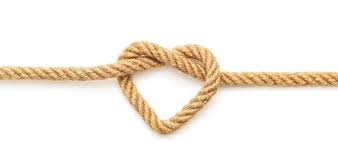
\includegraphics[width=7cm]{Pictures/images.jpg}
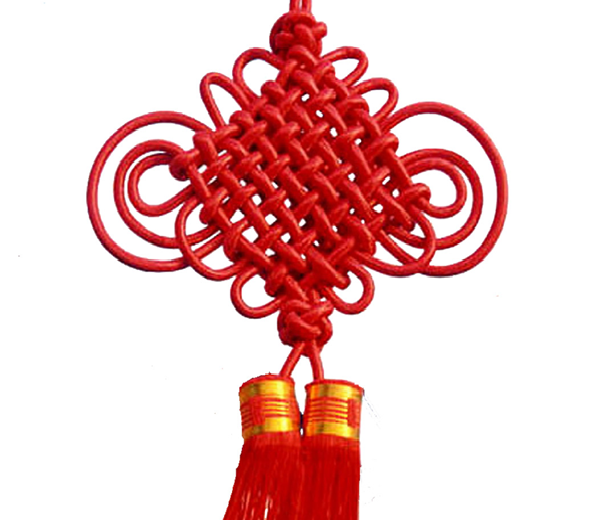
\includegraphics[width=3cm]{Pictures/chineseknot.png}

\end{frame}

% FRAME 2
\begin{frame}{What is a knot}
    \begin{itemize}
        \item Composite knots
    \end{itemize}
\centering
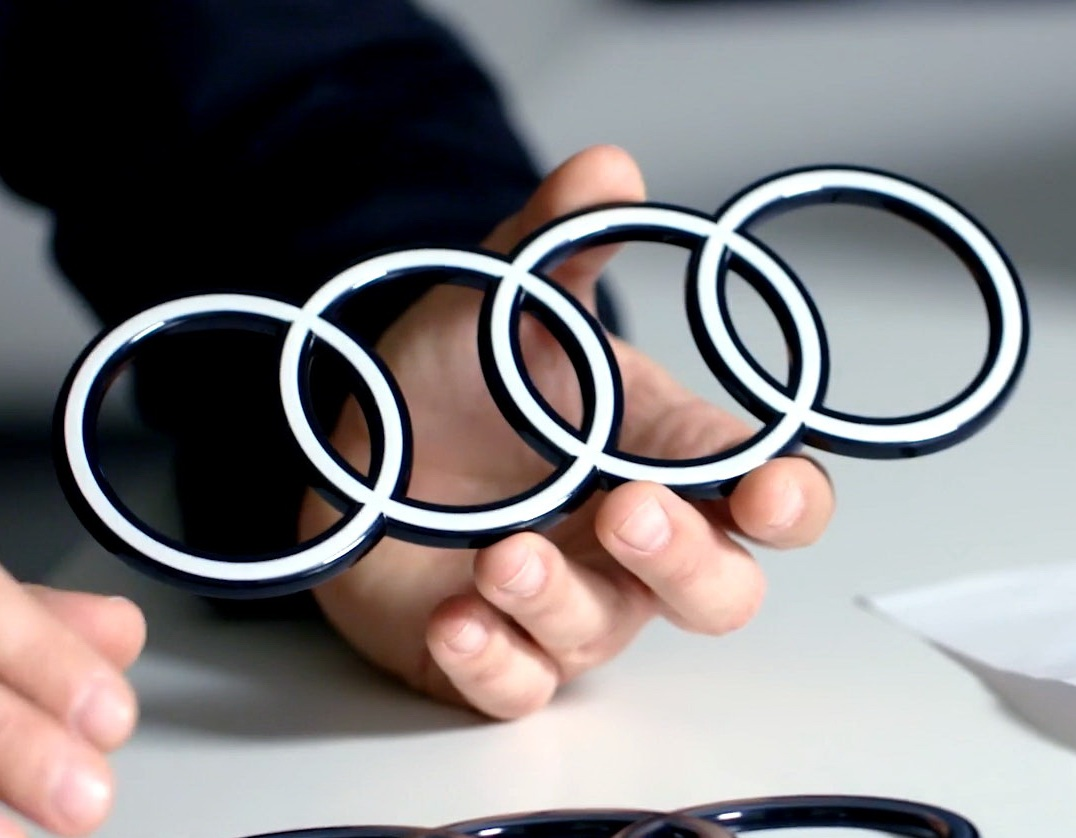
\includegraphics[width = 4.9cm]{Pictures/audi.jpg}
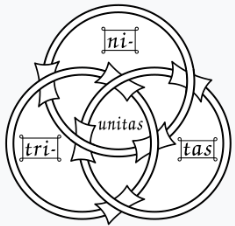
\includegraphics[width = 4cm]{Pictures/borromean.png}

\end{frame}

% FRAME 3 
\begin{frame}{What is a knot}
\begin{itemize}
    \item To study knots rigorously, we need to connect the two ends of the rope.
\end{itemize}
\begin{kulblock}{Definition}
    In mathematics, a knot is an embedding of the circle $\mathbf{S}^1$ into 3-dimensional Euclidean space, $\mathbf{R}^3$.
\end{kulblock}

\end{frame}

% FRAME 4
\begin{frame}{Motivation}
\begin{itemize}
    \item Peter Guthrie Tait and Lord Kelvin (19th century): During the research on composition of atoms, they conjectured that atoms are made out of vortex ring of ether.
\end{itemize}
\centering
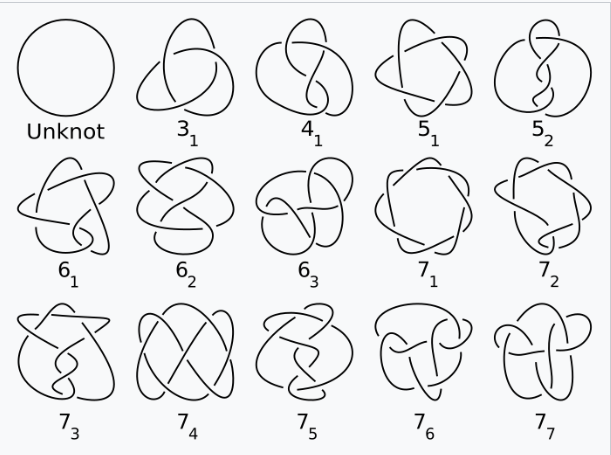
\includegraphics[width=5cm]{Pictures/simple knots.png}
\end{frame}

% FRAME 5
\begin{frame}{Motivation}
\begin{itemize}
    \item The structure of protein and DNA
\end{itemize}
\centering
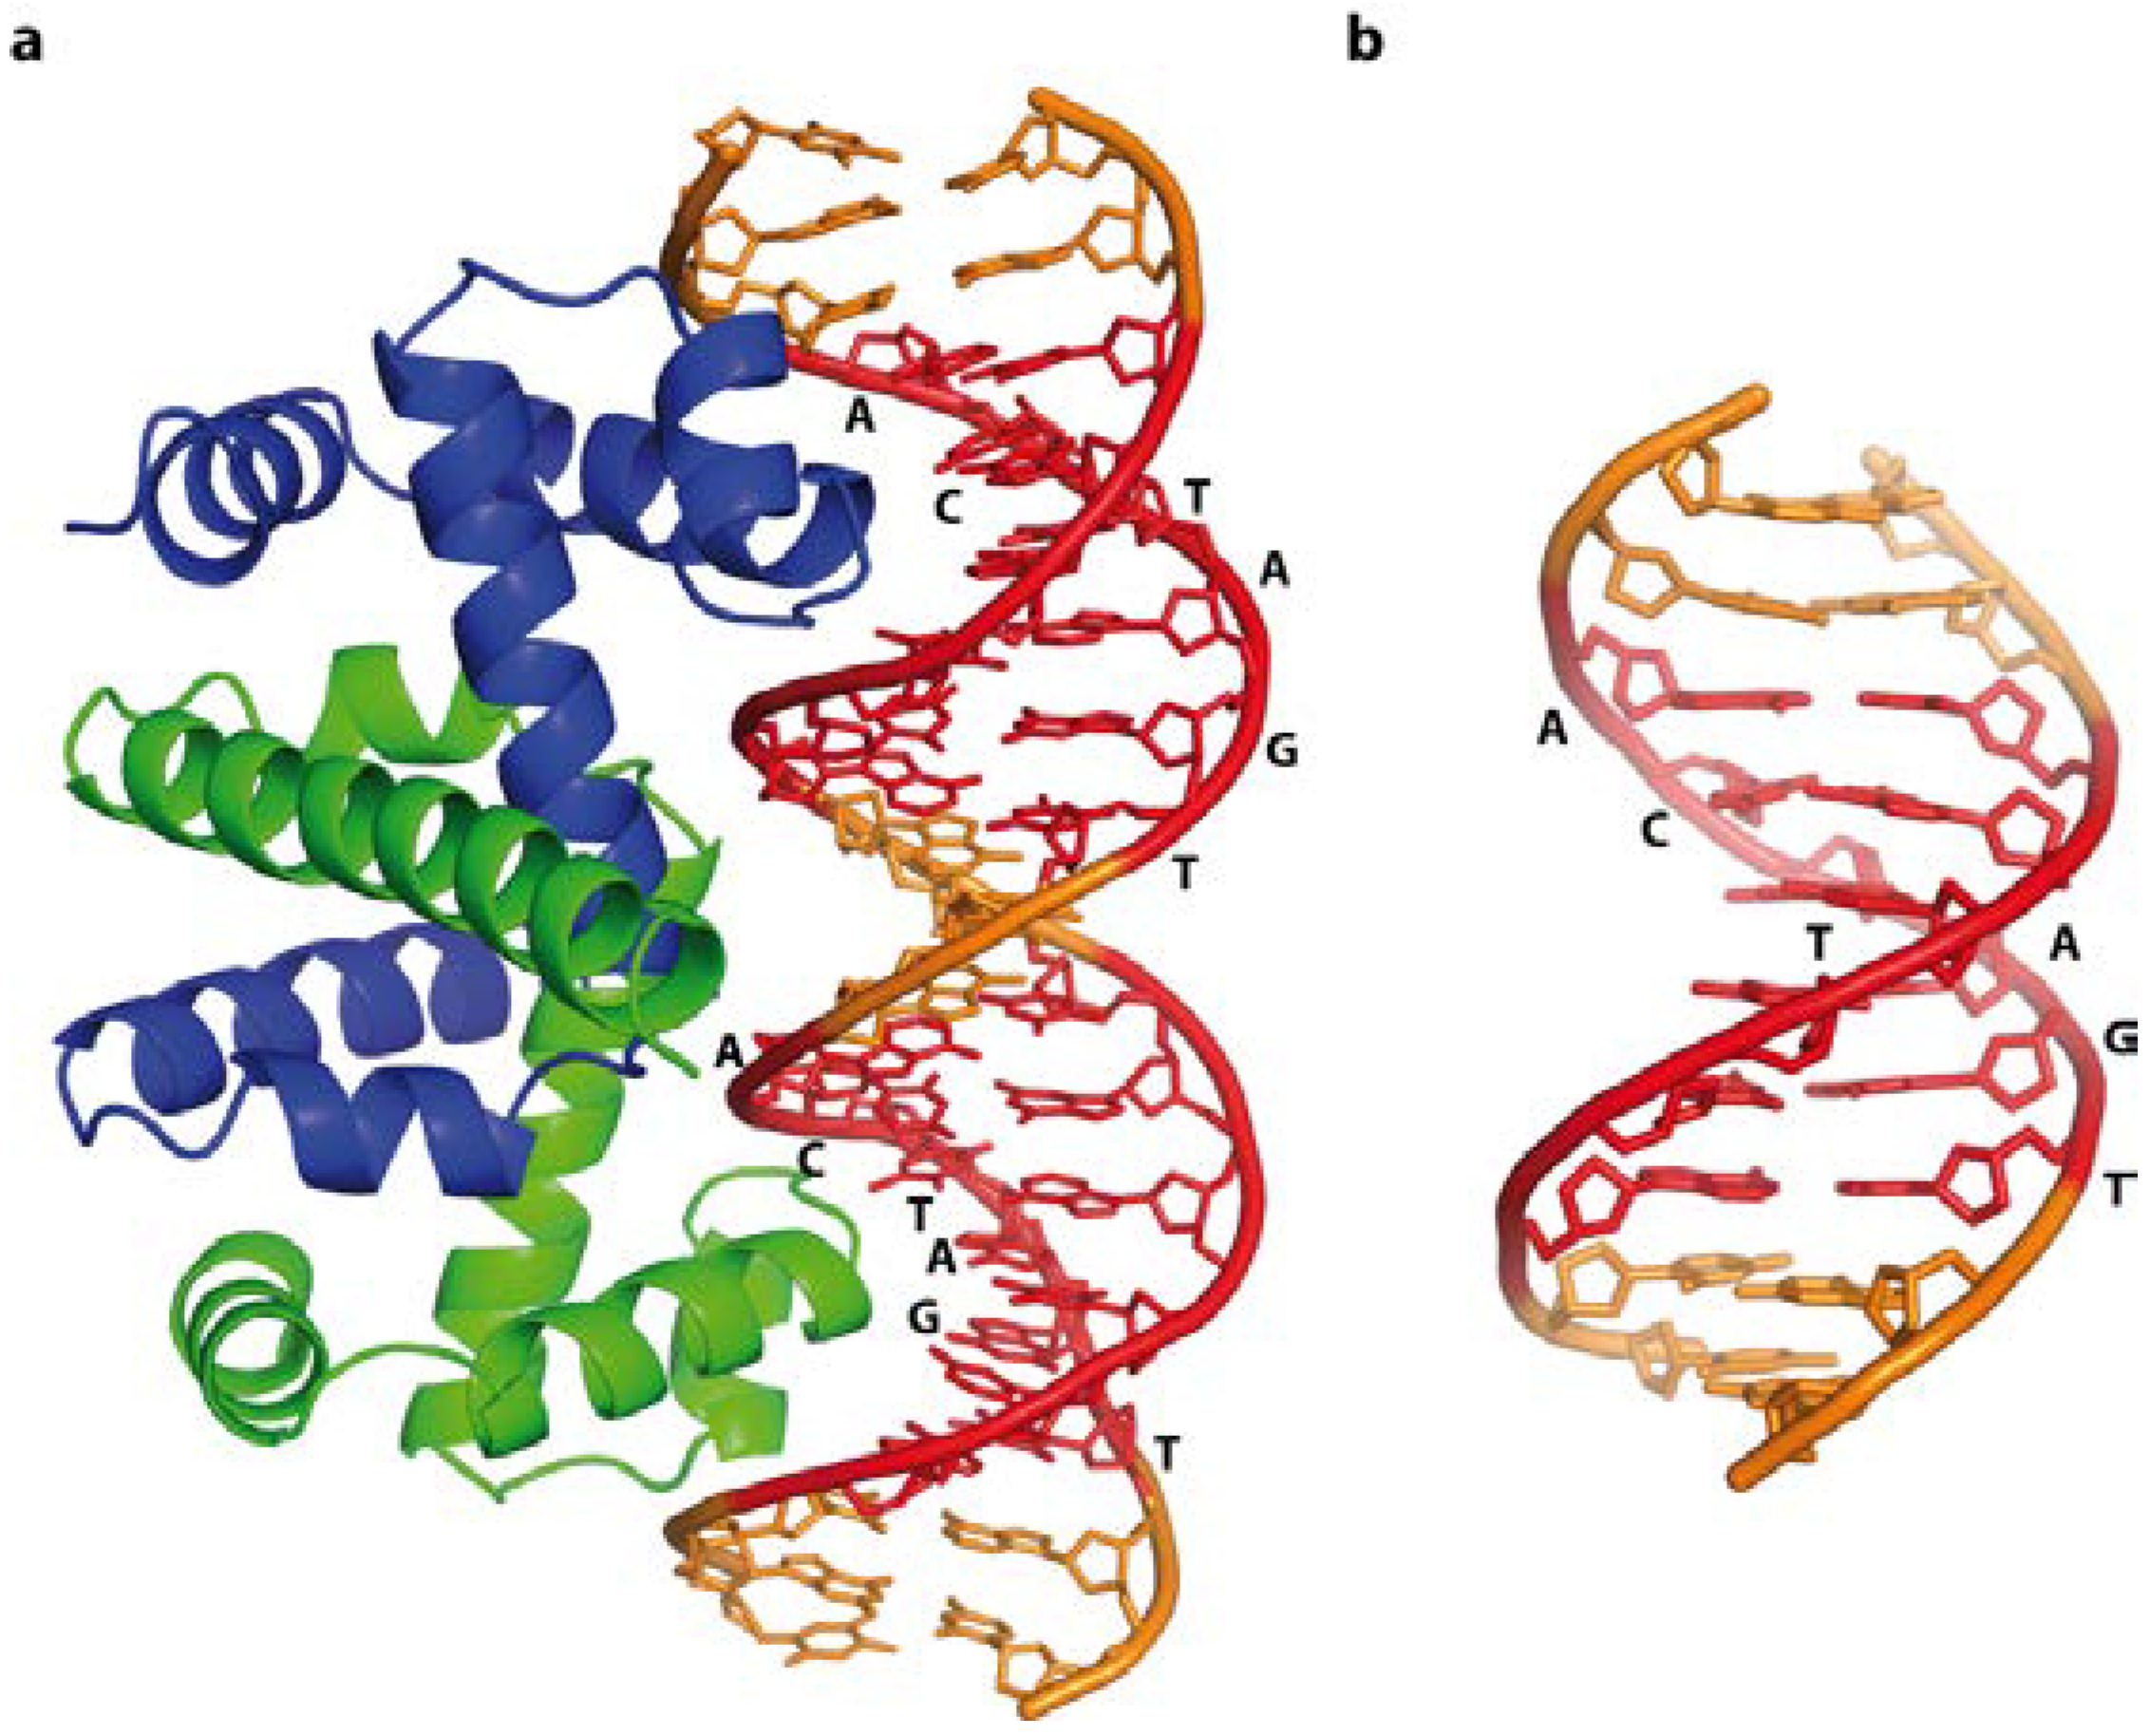
\includegraphics[width=7cm]{Pictures/DNA.png}
\end{frame}

% FRAME 6
\begin{frame}{Motivation}
\begin{itemize}
    \item The knot structure of chemical compound and material
\end{itemize}
\centering
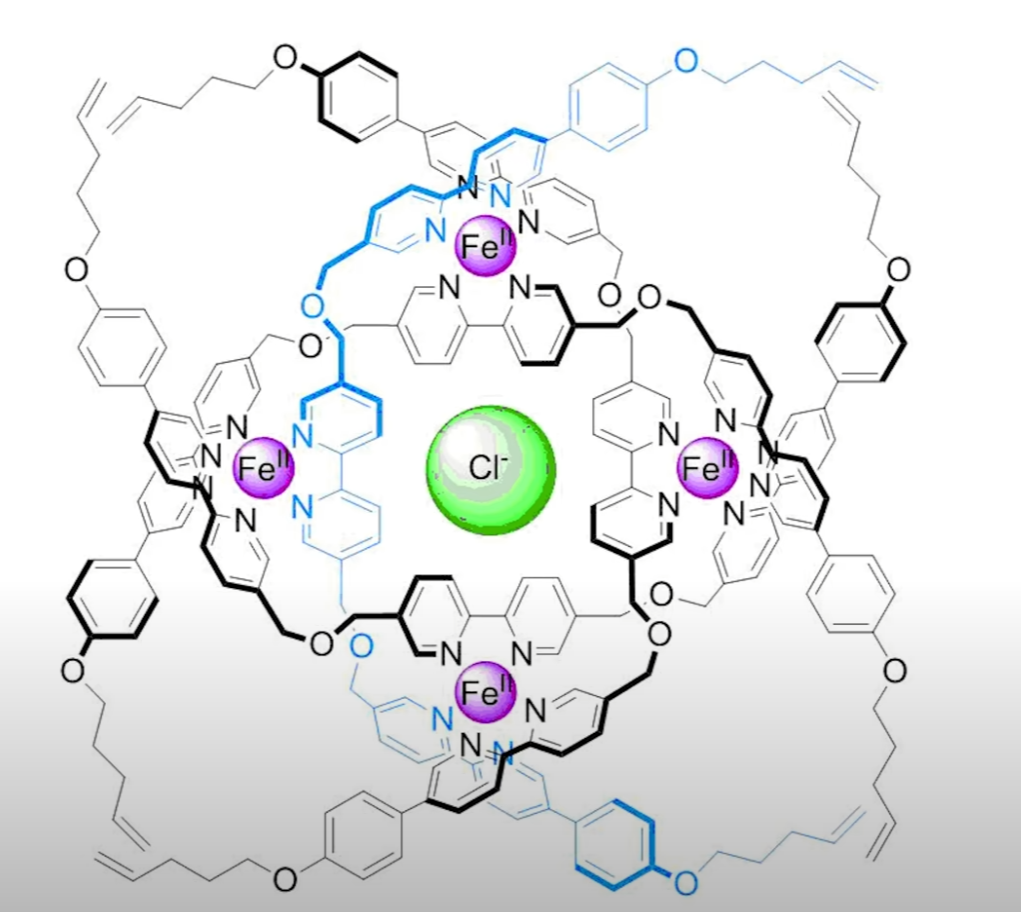
\includegraphics[width = 4.5cm]{Pictures/chemical.png}
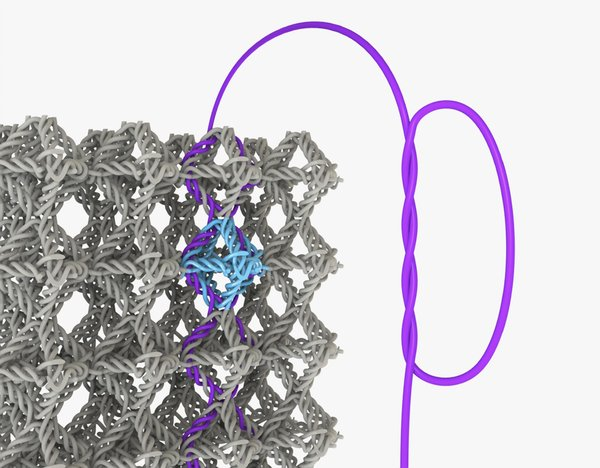
\includegraphics[width=4.5cm]{Pictures/material.jpg}
\end{frame}

% FRAME 7
\begin{frame}{Diagram}
\begin{itemize}
    \item How to represent a knot? Regular projection.
\end{itemize}
\begin{itemize}
    \item A knot projection is called a regular projection if no three points on the knot project to the same point, and no vertex
projects to the same point as any other point on the knot.
\end{itemize}
\end{frame}

% FRAME 8
\begin{frame}{Diagram}

\begin{itemize}
    \item A knot diagram is the regular projection of a knot to the plane with broken
lines indicating where one part of the knot undercrosses the other part.
\end{itemize}
\centering
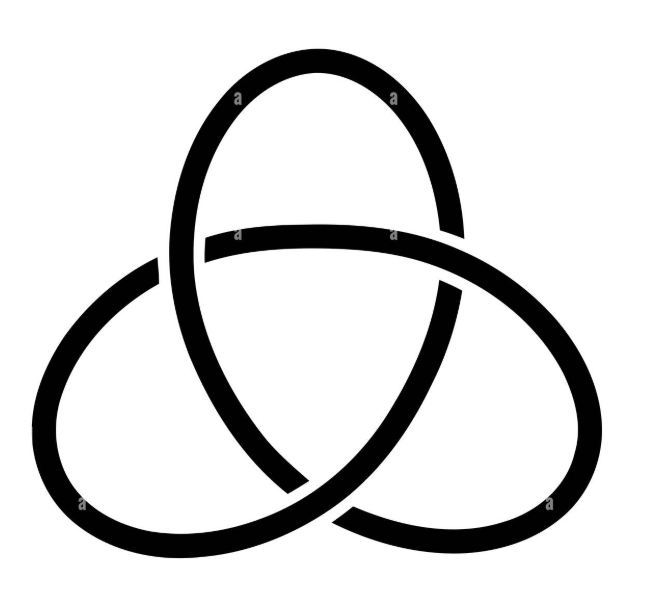
\includegraphics[width=3cm]{Pictures/trefoil.png}
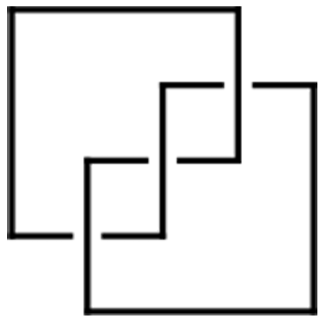
\includegraphics[width=3cm]{Pictures/31.png}
\end{frame}

% FRAME 9
\begin{frame}{Equivalence of knots}
\begin{itemize}
    \item Are they equivalent?
\end{itemize}
\centering
    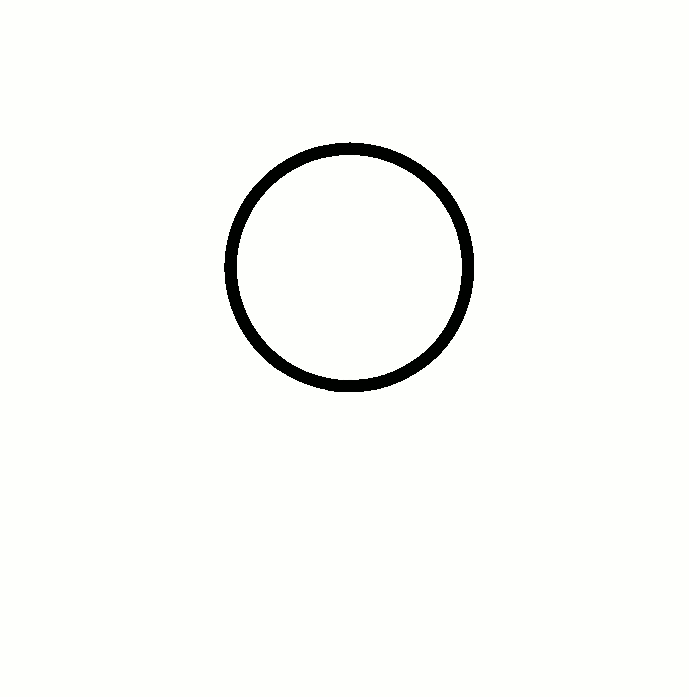
\includegraphics[width = 4cm]{Pictures/Simple.png}
    
\includegraphics[width = 4cm]{Pictures/complex.png}
\end{frame}


% FRAME 10
\begin{frame}{Reidemeister move}
\begin{itemize}
    \item Equivalence of knot?
\end{itemize}
\centering
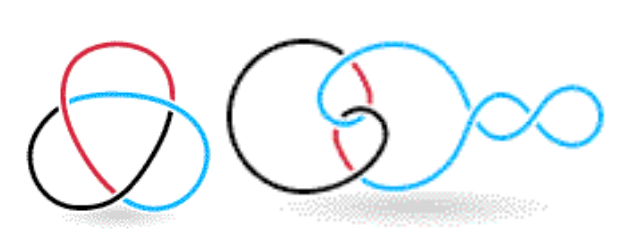
\includegraphics[width=7cm]{Pictures/equivalence.png}

\begin{itemize}
    \item Formal definition: two knots $\mathbf{K}_1$ and $\mathbf{K}_2$ are equivalent if there is an orientation-preserving homeomorphism $h:\mathbb{R}^3 \rightarrow \mathbb{R}^3$ with $h(\mathbf{K}_1) = h(\mathbf{K}_2)$.
\end{itemize}

\begin{itemize}
    \item Reidemeister's Theorem: If two knots are equivalent, their diagrams are related by a sequence of Reidemeister moves.
\end{itemize}
\end{frame}

% FRAME 11
\begin{frame}{Reidemeister move}
\begin{itemize}
    \item A Reidemeister move is an operation that can be performed on the diagram
of a knot whithout altering the corresponding knot.
\end{itemize}
\centering
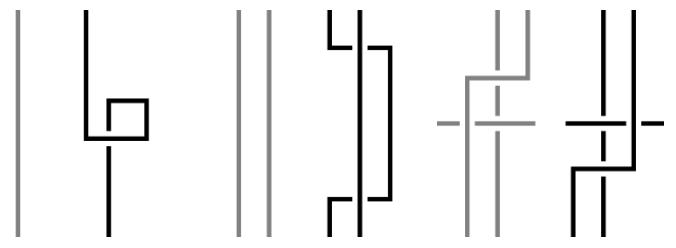
\includegraphics[width=7cm]{Pictures/r.png}
\end{frame}

% FRAME 12
\begin{frame}{Invariant polynomial}
    \begin{itemize}
        \item 1923(James Waddell Alexander): Alexander polynomial $\triangledown$. Reformulated by John Conway in 1969.
\centering
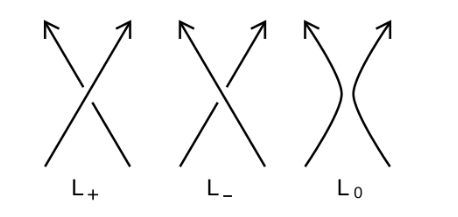
\includegraphics[width =7cm]{Pictures/L.png}
        $$\triangledown(O) = 1$$
        $$\triangledown(L^+) - \triangledown(L^-) = z\triangledown(L_0)$$
    \end{itemize}
\end{frame}

% FRAME 13
\begin{frame}{Invariant polynomial}
\begin{itemize}
    \item 1984(Vaughan Jones): Jones polynomial $V$. Jones won the field's medal for this discovery in 1990.
    $$V(L_0) = 1$$
    $$t^{-1}V(L_+) - tV(L_-) = (t^{\frac{1}{2}} - t^{-\frac{1}{2}})V(L_0)$$
    \item 1985(multiple authors): HOMFLY-PT polynomial $P$: A generalization of the above invariants.
    $$P(L_0) = 1$$
    $$tP(L_+) + t^{-1}P(L_-) + mP(L_0) = 0$$
\end{itemize}
\end{frame}

\section{Application of Knots}
\begin{frame}{Alternating Knots}
 In these types of knots, if you follow any strand in any direction you switch between upside and downside at any crossing.
\begin{figure}
    \centering
    
\includegraphics[height = 3.5cm, width= 8cm]{images/realalterknot.png}
    \caption{An alternating knot}
    \label{alterknot}
\end{figure}
\cite{https://doi.org/10.1002/anie.201702531}
\end{frame}
\begin{frame}{Rational Knots}
Rational knots are obtained by closing off the edges of rational tangles. A tangle is a region in a knot that is separated from the knot by a circle and has four outgoing strands crossing the circle. 
\begin{figure}[h]
    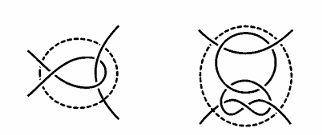
\includegraphics[width=0.6\linewidth]{images/tangles.png}
    \caption{Tangles}
    \label{tangles}
\cite{adams2004knot}
\end{figure}
\end{frame}
\begin{frame}
\begin{columns}[T]
\begin{column}{.48\textwidth}
\begin{figure}
    \centering
    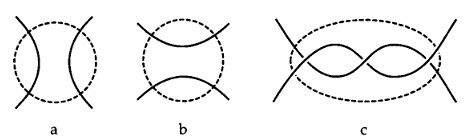
\includegraphics[width=0.9\linewidth,height=4cm]{images/basictangles.png}
    \caption{$\infty$, 0 and 3 tangles, they are \centering fundamental}
    \label{basictangles}
\end{figure}
\cite{adams2004knot}
\end{column}
\begin{column}{.48\textwidth}
\begin{figure}[h]
    \centering
    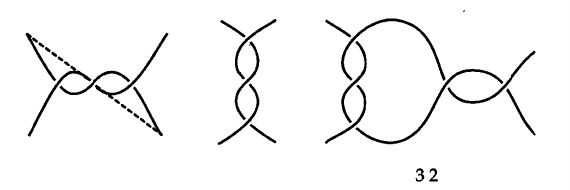
\includegraphics[width=0.9\linewidth,height=4cm]{images/tangleproduce.png}
    \caption{Generating Tangles}
    \label{generating}
\end{figure}
\end{column}
\end{columns}
\end{frame}
\begin{frame}{Pretzel Knots}
Pretzel knots are rational knots that are obtained by adding up rational tangles. If every term of a rational knot klm (for instant 311) is multiplied with 0 and then added altogether, the result is a pretzel knot that is denoted by k,l,m (3,1,1)
\begin{figure}
    \centering
    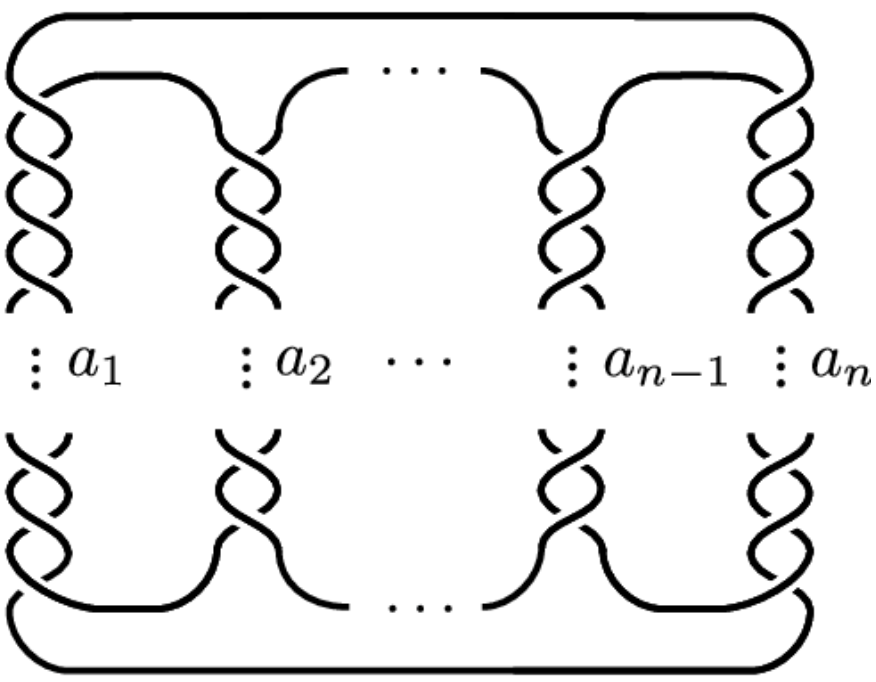
\includegraphics[width=0.4\linewidth]{images/pretzel.png}
    \label{pretzel}
    \cite{article2}
\end{figure}
\end{frame}
\begin{frame}{Torus Knots}
These knots are wrapped around unknotted tori and do not cross themselves as they move around their tori. There are 'short' paths called meridian and 'long' paths called longitude. A (p,q)-torus knot travels the longitude p times and travels meridians q times.
\begin{figure}
    \centering
    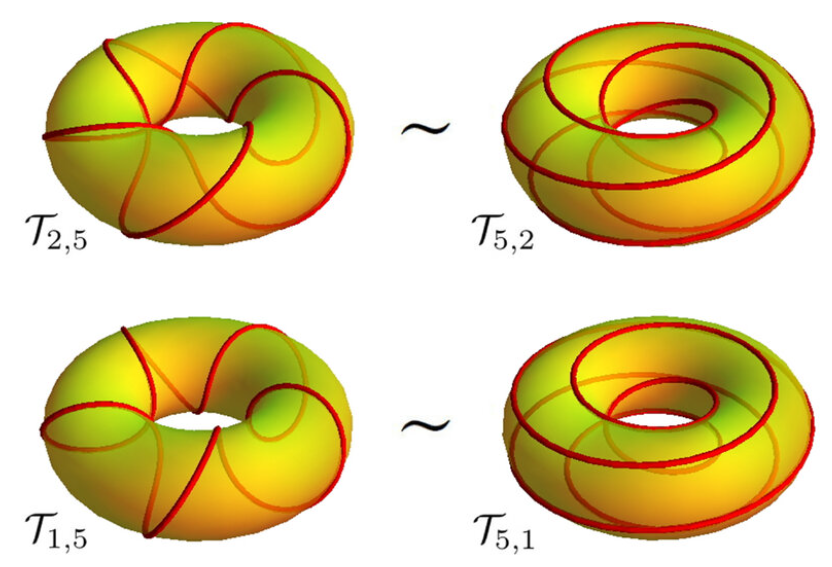
\includegraphics[height= 4cm, width=8cm]{images/torus.png}
    \label{torus}
   
\end{figure}
\cite{article}    
\end{frame}
\begin{frame}{Knots and Biology}
\begin{columns}[T]
\begin{column}{.48\textwidth}
\cite{555w}
\begin{figure}
    \centering
    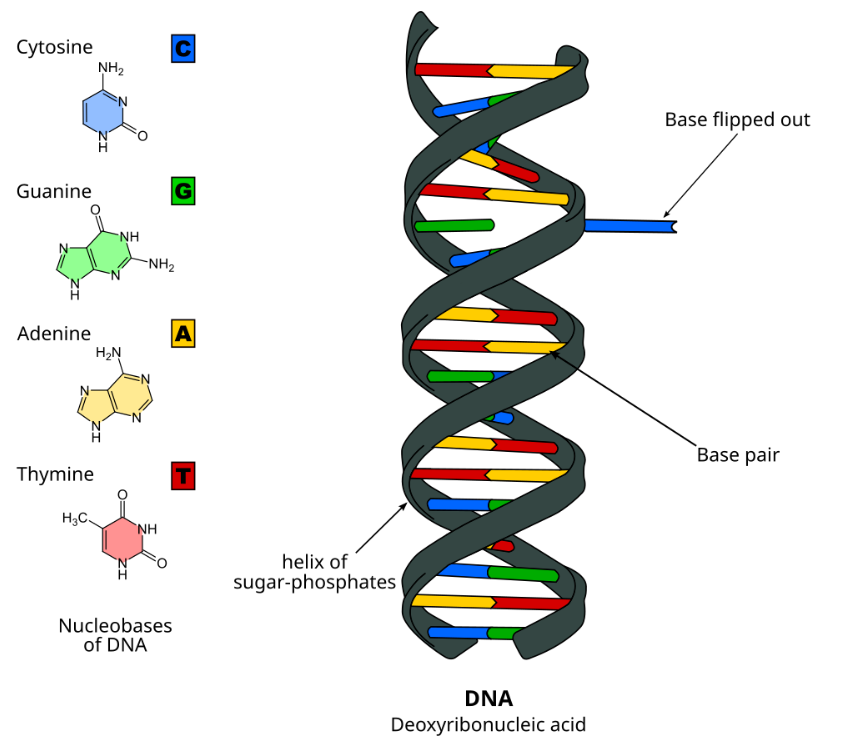
\includegraphics[width= 6cm,height=5.5cm]{images/dnastring.png}
    \label{dnast}
\end{figure}
\end{column}
\begin{column}{.48\textwidth}
\cite{adams2004knot}
\begin{figure}[h]
    \centering
    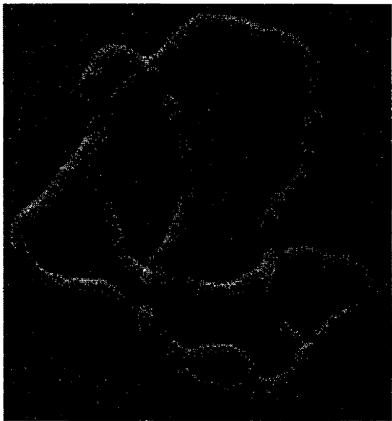
\includegraphics[width= 6cm,height=5.5cm]{images/electron.png}
    \label{elec}
\end{figure}
\end{column}
\end{columns}
\end{frame}
\begin{frame}
\begin{columns}[T]
\begin{column}{.48\textwidth}
\begin{itemize}
    \item \bold{Tw(R)}: Twist of the ribbon. Average of crossings over the axis
    \item \bold{Wr(R)}: Writhe of the ribbon. Average of crossings of the axis from every projection it is \\ \vspace{0.2cm} $\frac{\int signed-crossover-number.dA }{\int dA}$
    \item \bold{Lk(R)}: Linking number
    \item \bold{Lk(R) = Tw(R) + Wr(R)}
\end{itemize}
\end{column}
\begin{column}{.48\textwidth}
\begin{figure}
    \centering
    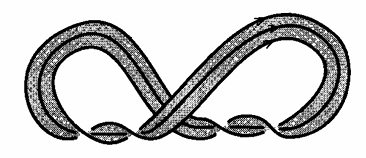
\includegraphics[width=0.6\linewidth]{images/ribbon.png}
    \caption{Axis}
    \label{axis}
    \cite{adams2004knot}
\end{figure}
\begin{figure}
    \centering
    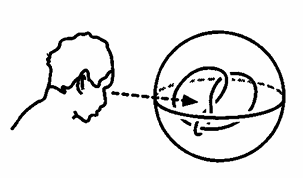
\includegraphics[width=0.6\linewidth]{images/vantage.png}
    \label{vantage}
    \cite{adams2004knot}
\end{figure}
\end{column}
\end{columns}
    
\end{frame}
\begin{frame}
\begin{columns}[T]
\begin{column}{.48\textwidth}
\begin{itemize}
\item S: Substrat tangle
\item T: Site tangle
\item R: Recombination tangle
\item N(Q): Converting tangle to a knot or a link
\item N(S + T) = N(1) (unknot)
\item N(S + R) = N(2) (Hopf link)
\item N(S + R + R) = N(211) (figure-eight knot)
\item N(S + R + R + R) = N(11111) (Whitehead link)
\end{itemize}
\end{column}
\begin{column}{.48\textwidth}
\begin{figure}
    \centering
    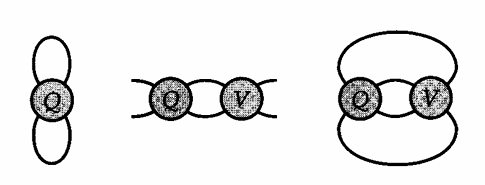
\includegraphics[width=1\linewidth]{images/subtang.png}
    \label{subtang}
    \cite{adams2004knot}
\end{figure}
\begin{figure}
    \centering
    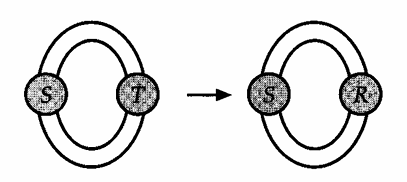
\includegraphics[width=0.75\linewidth]{images/substrat.png}
    \label{substrat}
    \cite{adams2004knot}
\end{figure}
\end{column}
\end{columns}
\end{frame}
\begin{frame}
\begin{figure}
    \centering
    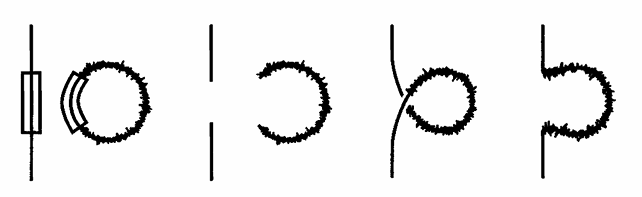
\includegraphics[width=0.6\linewidth]{images/inten.png}
    \label{inten}
\end{figure}
\begin{figure}
    \centering
    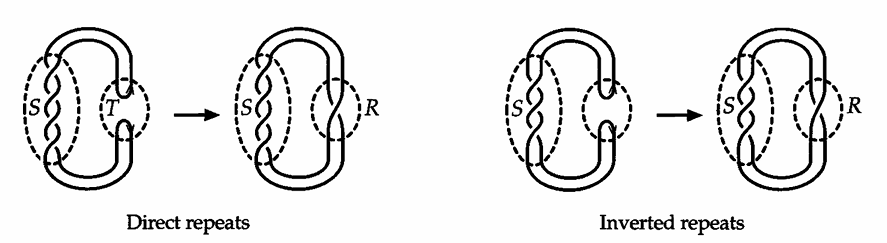
\includegraphics[width=0.75\linewidth]{images/inten2.png}
    \caption{Effects of Int enzyme}
    \label{inten2}
    \cite{adams2004knot}
\end{figure}   
\end{frame}
\begin{frame}{Knots and Chemistry}
\begin{columns}[T]
\begin{column}{.48\textwidth}
\begin{figure}
    \centering
    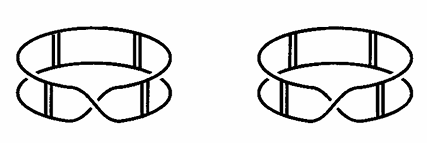
\includegraphics[width=0.8\linewidth]{images/mobius.png}
    \caption{Homeomorphic but not isotopic \centering molecules}
    \label{mobius}
    \cite{adams2004knot}
\end{figure}
\end{column} 
\begin{column}{.48\textwidth}
\begin{figure}
    \centering
    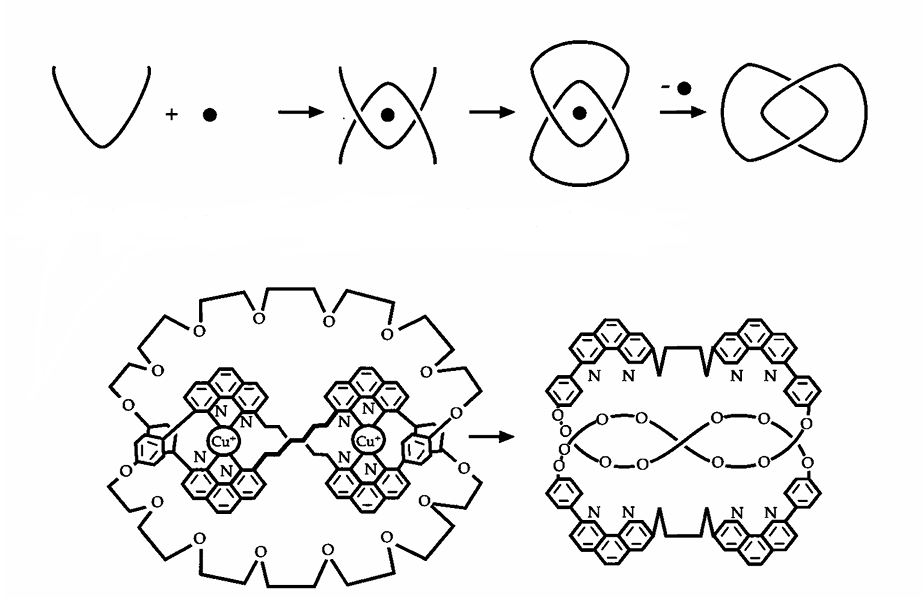
\includegraphics[width=0.9\linewidth]{images/mergedmolecule.png}
    \label{merged}
    \cite{adams2004knot}
\end{figure}
\end{column}
\end{columns}
\end{frame}
\begin{frame}{Knots and Topology}
Poincaré Conjecture: Every three-dimensional topological manifold which is closed, connected, and has trivial fundamental group is homeomorphic to the three-dimensional sphere.
\begin{figure}
    \centering
    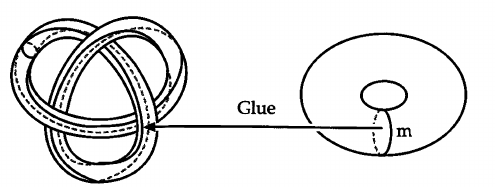
\includegraphics[width=0.5\linewidth]{images/dehn.png}
    \caption{Dehn Surgery}
    \label{dehn}
    \cite{adams2004knot}
\end{figure}
\end{frame}
\begin{frame}{Open Problems}
    \begin{itemize}
        \item Could there be a constant c such that for any knot K and for any two projections P 1 and P2 of K, each with no more than n crossings, one can get from one projection to the other by Reidemeister moves without ever having more than n + c crossings at any intermediate stage?
        \item Find all of the 14-crossing prime knots.
        \item Show that the number of distinct prime (n + 1)-crossing knots is
greater than the number of distinct prime n-crossing knots, for each
positive integer n.
        \item Is it true that a knot with
unknotting number n cannot be a composite knot with n + 1 factor
knots?
\item Show that the crossing number of a composite knot is the sum of the
crossing numbers of the factor knots, that is, $c(K_1#K_2) = c(K_1) + c(K_2)$
    \end{itemize}
    \cite{adams2004knot}
\end{frame}

\section{Fractals}

\begin{frame}
	\frametitle{Application}
	\begin{itemize}
		\item Medicine
		\begin{itemize}
			\item Identifying tumors in brain MR images \cite{iftekharuddin2003fractal}
			\item Diabetic retinopathy, etc. : blood vessel's diameter \cite{uahabi2015applications}
		\end{itemize}
		\item Economics
	\end{itemize}
\end{frame}

\section[]{Embedding into Menger Sponge}
\begin{frame}{The Menger Sponge}
\begin{itemize}
    \item Universal - Contains every curve
\end{itemize}
    \begin{figure}
        \centering
        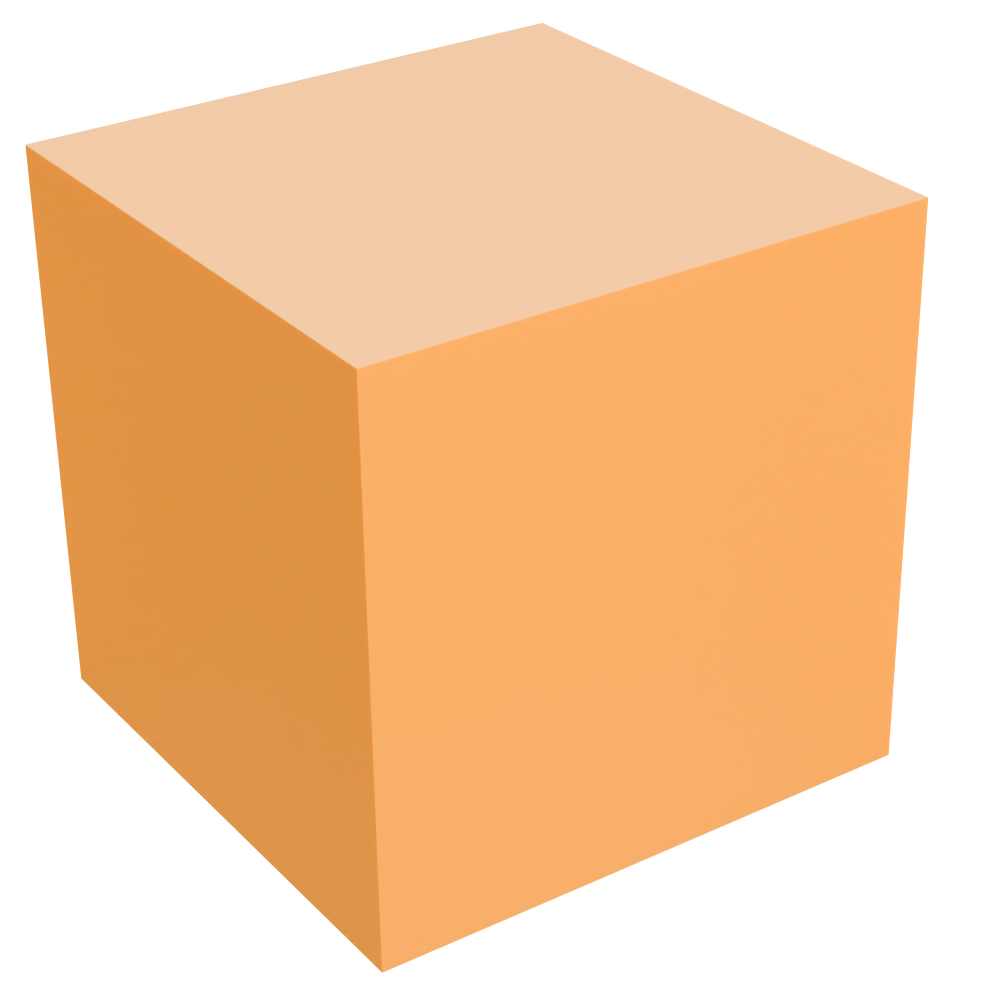
\includegraphics[width=0.25\linewidth]{MichaelImages/Cube.png}
        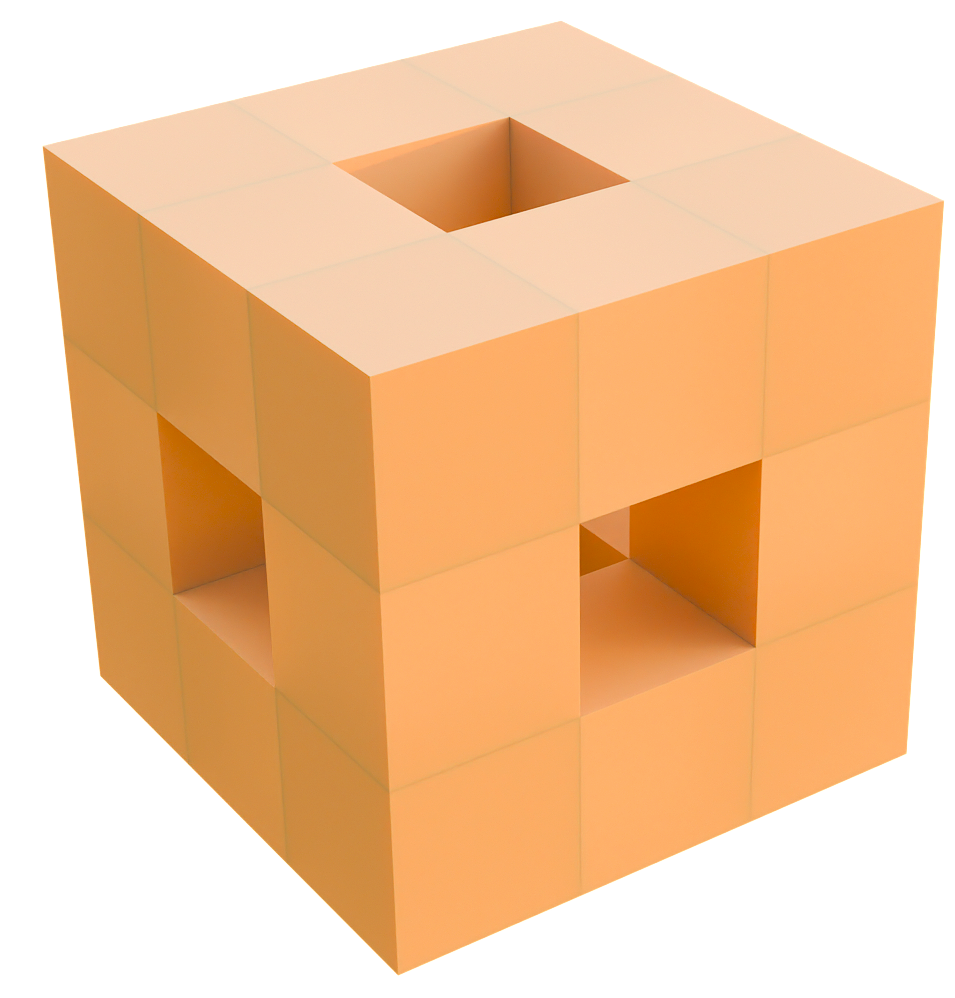
\includegraphics[width=0.25\linewidth]{MichaelImages/FirstIterationCube.png}
         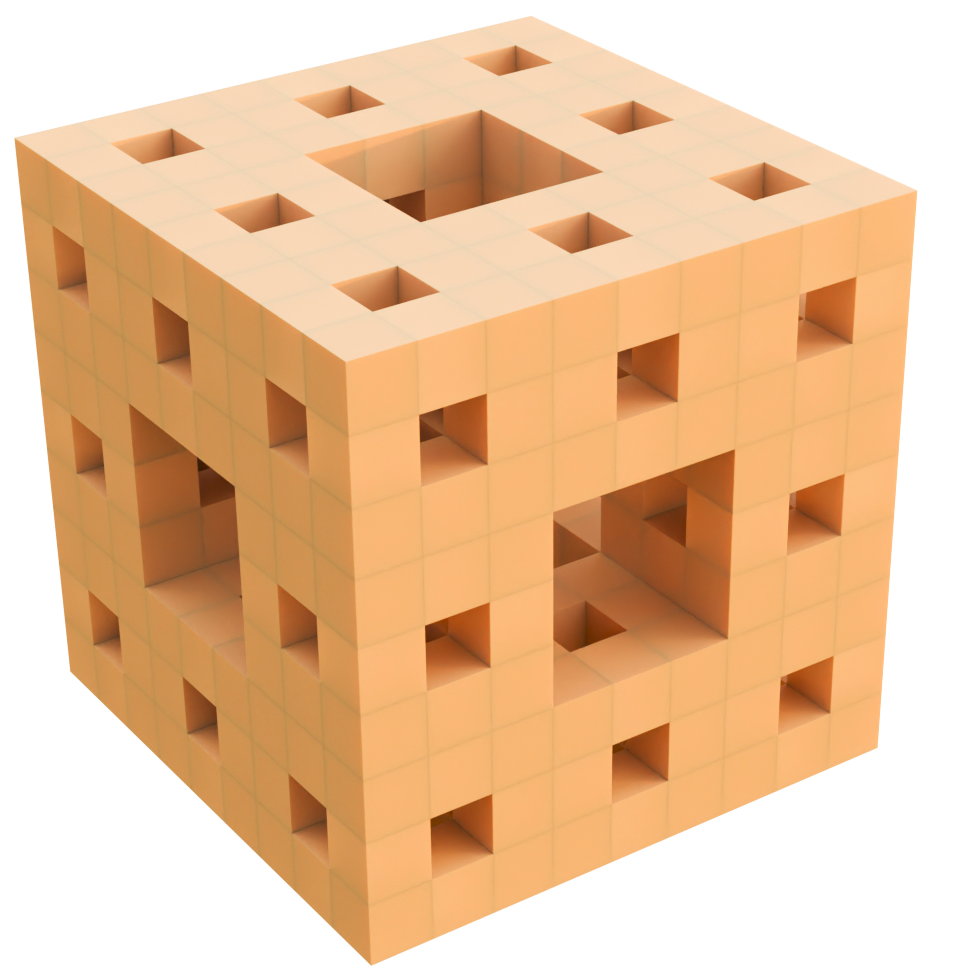
\includegraphics[width=0.25\linewidth]{MichaelImages/SecondIterationCube.png}
        \caption{Michael McGloin (2025)}
        \label{fig:enter-label}
    \end{figure}
\end{frame}

\begin{frame}{Knots Inside the Menger Sponge}
    What is a knot in the Menger Sponge?
    \begin{figure}
        \centering
        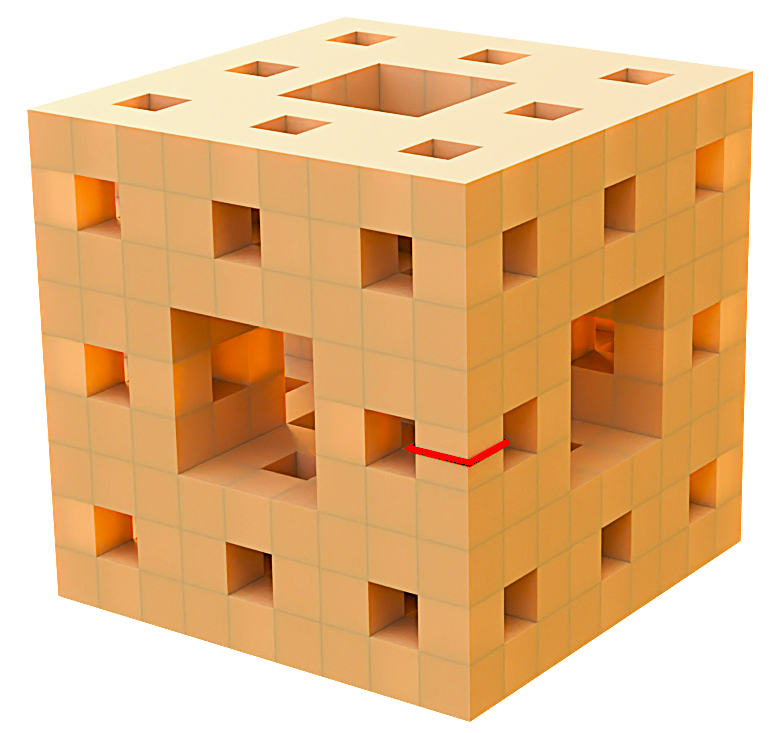
\includegraphics[width=0.35\linewidth]{UnknotTwo.png}
        \caption{The Unknot? - Michael McGloin (2025)}
        \label{fig:enter-label}
    \end{figure}
\end{frame}
\begin{frame}{Not a Knot!}
\begin{figure}
    \centering
    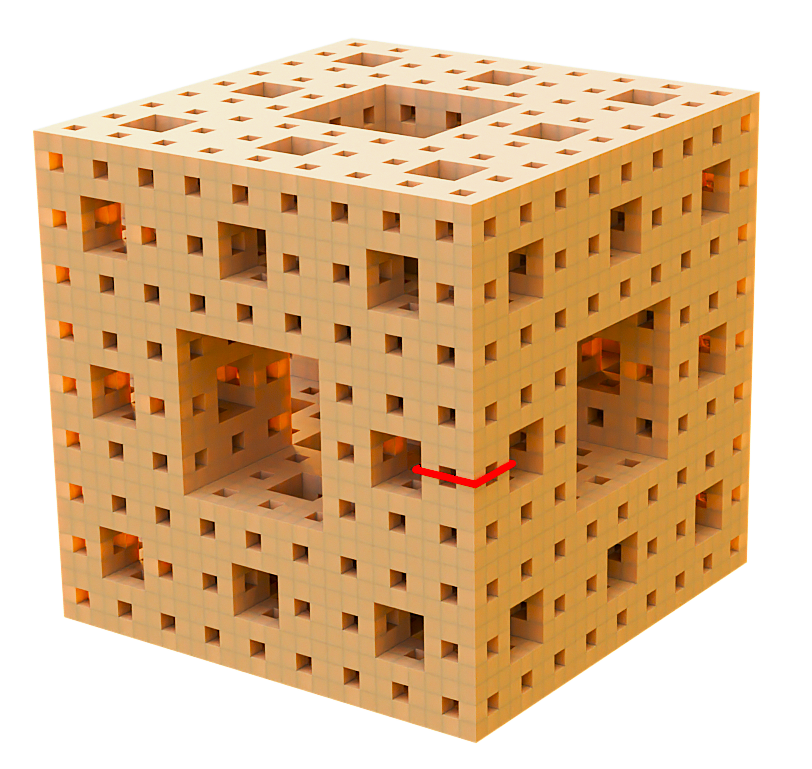
\includegraphics[width=0.49\linewidth]{NotAKnot.png}
    \label{fig:enter-label}
\end{figure}
\end{frame}

\begin{frame}{Knot or Not?}
\begin{itemize}
    \item Does the following knot live on the fractal?

    \begin{figure}
        \centering
        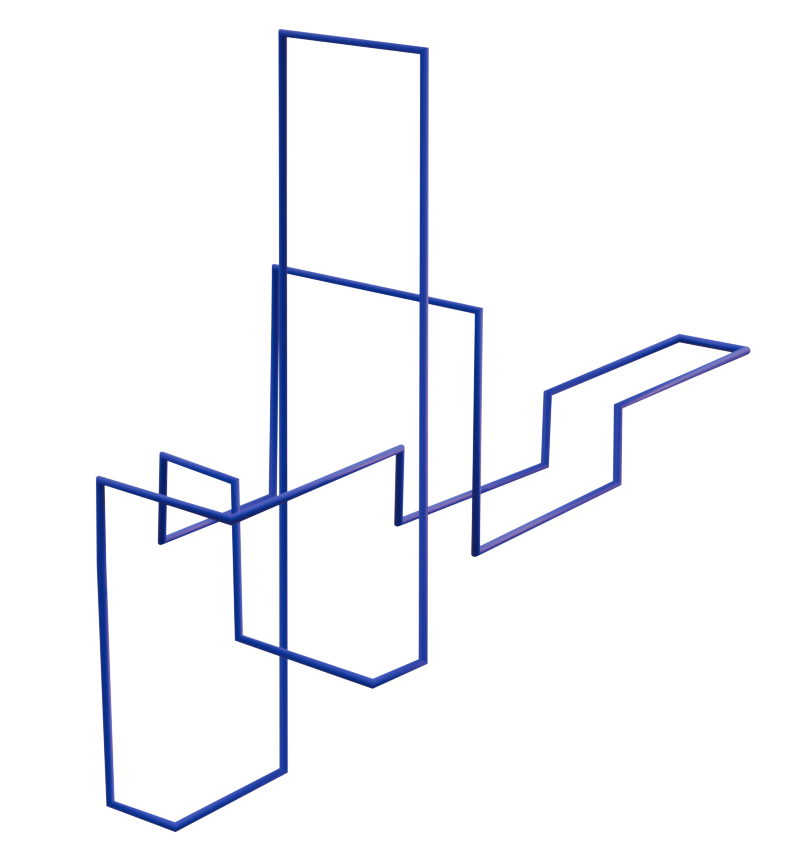
\includegraphics[width=0.25\linewidth]{NoCubeTrefoil.png}
        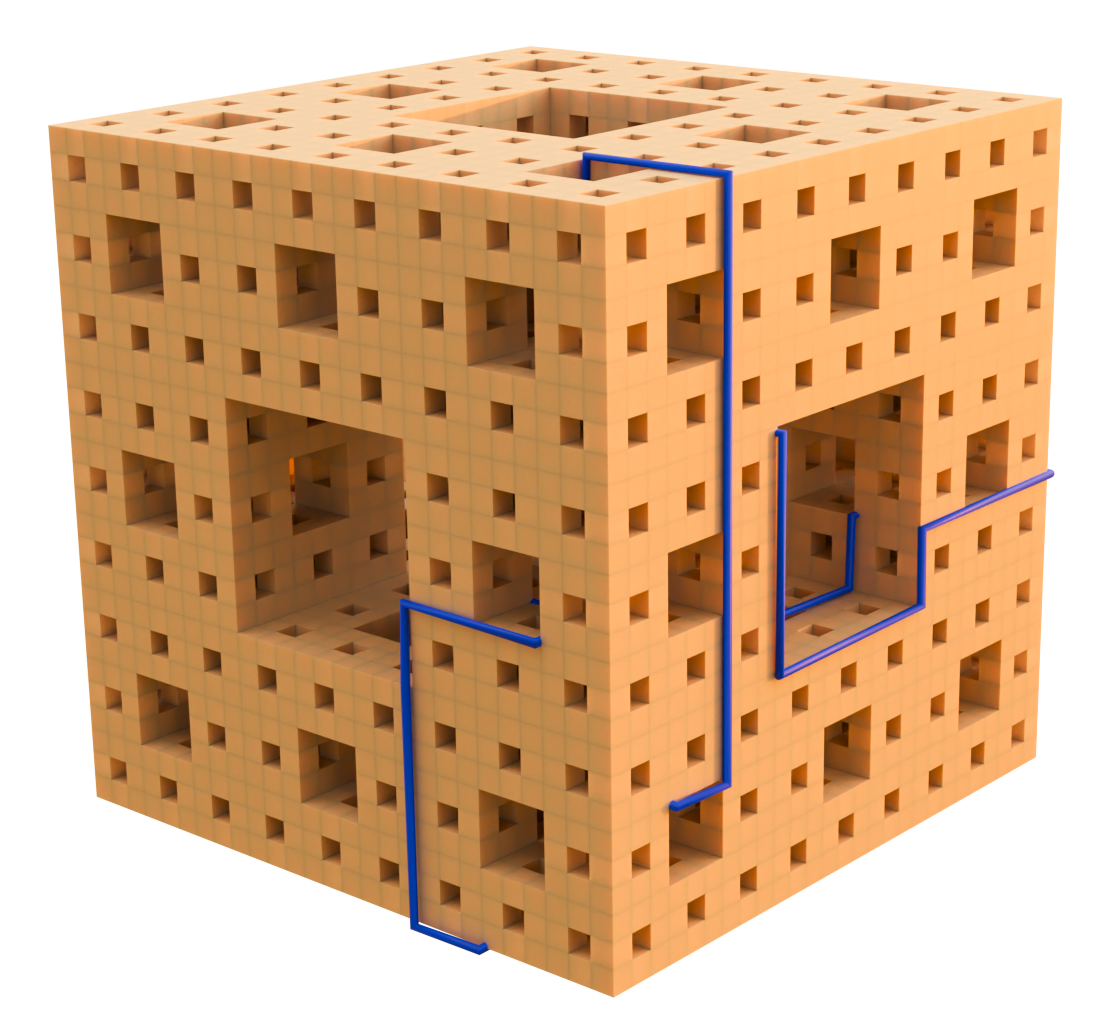
\includegraphics[width=0.3\linewidth]{TreFoilKnot.png}
        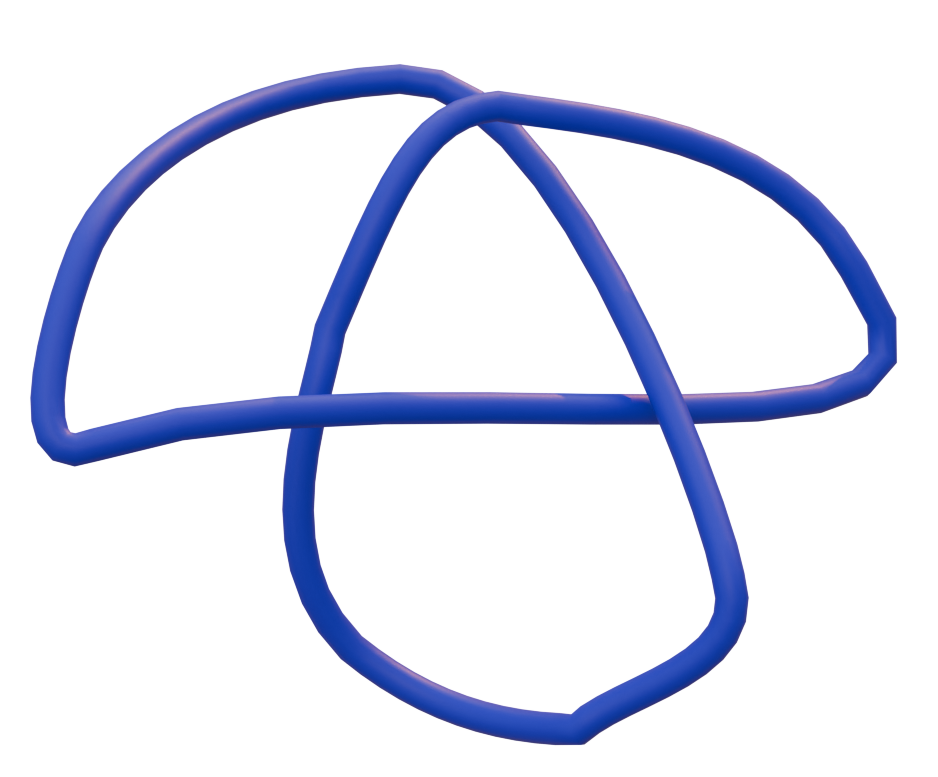
\includegraphics[width=0.3\linewidth]{UnravelledTrefoil.png}
        \caption{Trefoil Knot in Sponge - Michael McGloin (2025)}
        \label{fig:enter-label}
    \end{figure}
    \item What possible knots can we find in this fractal?
\end{itemize}
\end{frame}

\begin{frame}{The Positive Answer}
\begin{center}
    This is the question asked by highschoolers Niko Voth (top right), Joshua Broden (bottom right) and Noah Nazareth under the supervision of Malors
\end{center}
\begin{itemize}
    \item In 2024 they were able to show that you could find every possible knot embedded in the Menger Sponge!
    \item Published a paper on ArXiv.    
\end{itemize}
 \begin{figure}
     \centering
     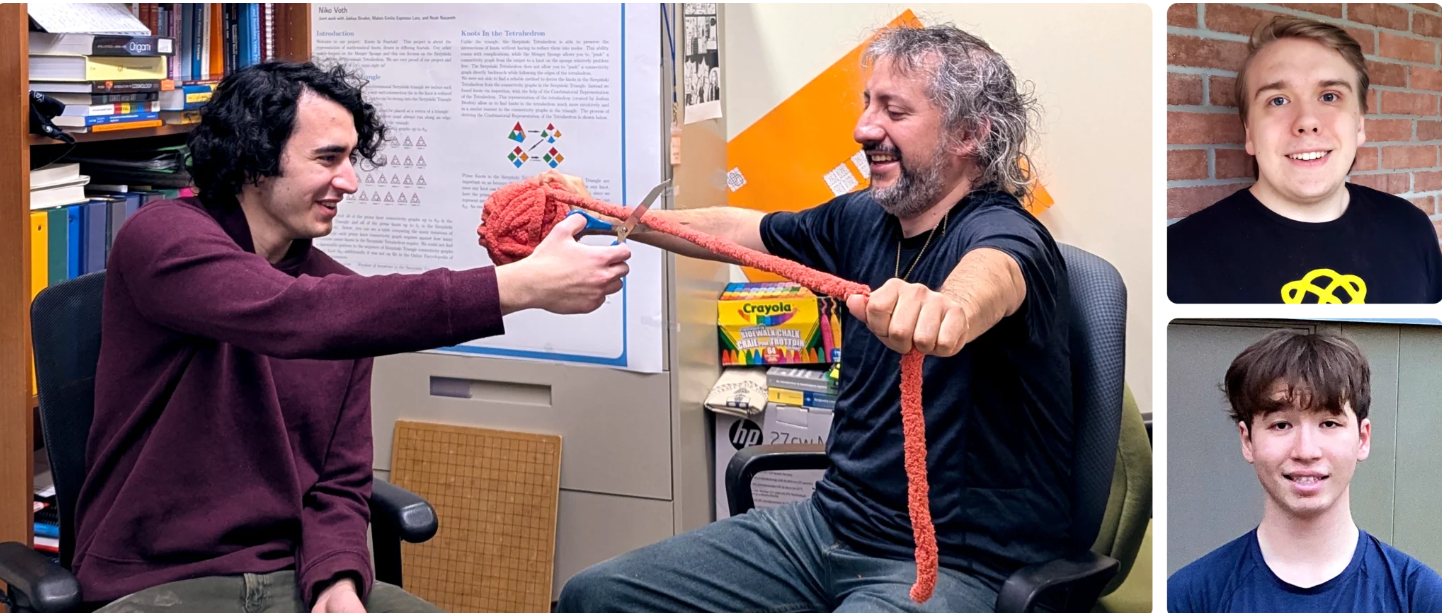
\includegraphics[width=0.5\linewidth]{PhotoOfAuthors.png}
     \caption{\cite{Quanta}}
     \label{fig:enter-label}
 \end{figure}
\end{frame}

\begin{frame}{The Cantor Set}
\begin{itemize}
    \item Split the interval $[0,1]$ into thirds and remove the middle third
    \item Repeat on each remaining interval
\end{itemize}
\begin{remark}
    A point $x \in [0,1]$ is in the Cantor set if it does not have a 1 in its ternary expansion.
\end{remark}
\begin{figure}
    \centering
    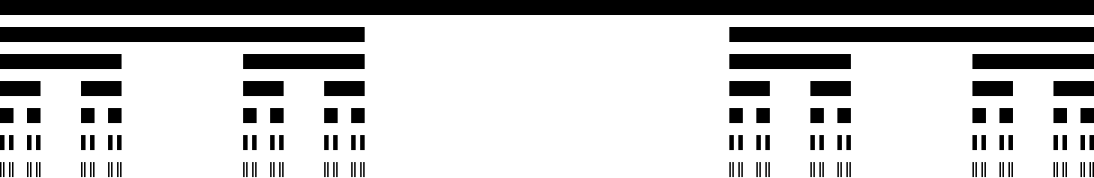
\includegraphics[width=0.5\linewidth]{Cantor_set_in_seven_iterations.svg.png}
    \caption{Cantor Set - \cite{cantor}}
    \label{fig:enter-label}
\end{figure}
\end{frame}

\begin{frame}{Cantor Dust}
Cantor dust is a 2 dimensional fractal and is the cartesian product of 2 cantor sets
 \begin{figure}
     \centering
     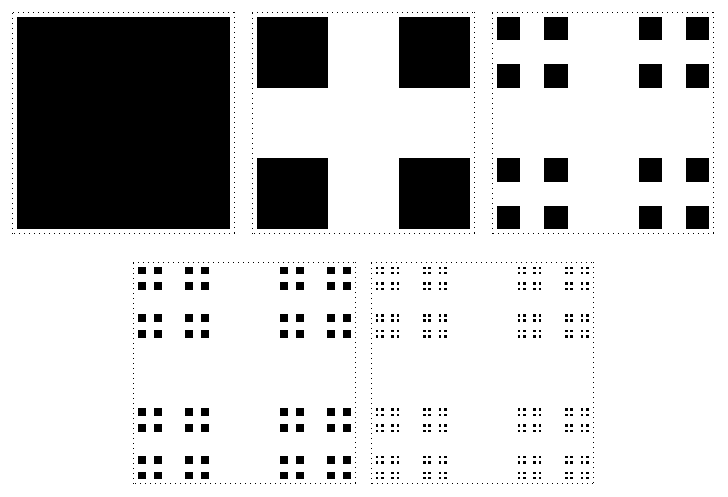
\includegraphics[width=0.5\linewidth]{cantordust.png}
     \caption{\cite{555w}}
     \label{fig:enter-label}
 \end{figure}
\end{frame}

\begin{frame}{Relation With Sierpienski Carpet}
Cantor dust is a 2 dimensional fractal and is the cartesian product of 2 cantor sets
 \begin{lemma}
     $(x,y)$ lies on the Sierpinski carpet if and only if $x$ and $y$ share no digit $1$ in their ternary expansion.
 \end{lemma}
\begin{figure}
    \centering
    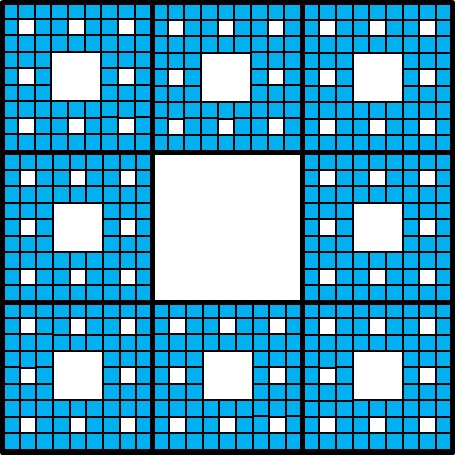
\includegraphics[width=0.2\linewidth]{Carpet.jpg}
    \caption{\cite{sierpinski2016}}
    \label{fig:enter-label}
\end{figure}
\end{frame}

\begin{frame}{Which Points Lie on the Menger Sponge?}
\begin{lemma}
    Let $ (x, y)$ be a Cantor Dust point, then $(x,y,z) \in M$ for all $0 \leq z \leq 1$.
\end{lemma}

\begin{proof}
Consider the first 2 stages where regions not in black have a hole behind them. 
    \begin{figure}
        \centering
        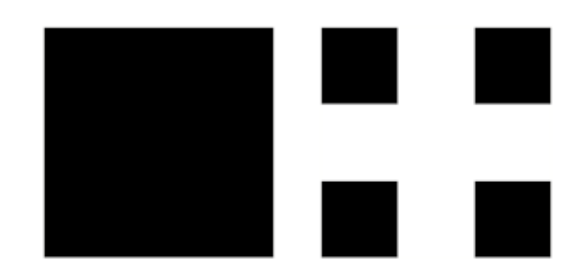
\includegraphics[width=0.22\linewidth]{ProofOfPointsOnSponge.png}
        \caption{Stage 0 and Stage 1 \cite{broden2024knotsinsidefractals}}
        \label{fig:enter-label}
    \end{figure}
\end{proof}
\end{frame}

\begin{frame}{Which Points Lie on the Menger Sponge?}
\begin{proof}[Proof (Cont.)]
\begin{itemize}
    \item In the next iteration of the sponge we need only consider the black regions as it is never possible to fill in a hole. 
    \item However, each black region occurs at a square of dimension $\frac{1}{3}\times\frac{1}{3}$ and so can be viewed as Stage $0$ when zoomed in. 
    \item Repeating this argument inductively we see that the black areas precisely align with points of the Cantor Dust fractal.
\end{itemize}
\end{proof}
\begin{figure}
        \centering
        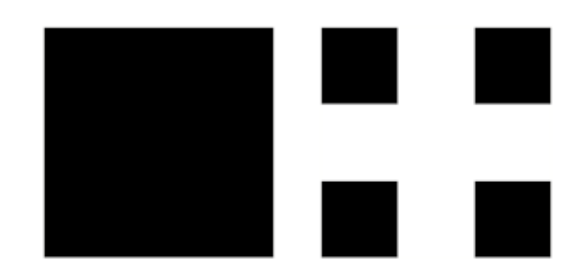
\includegraphics[width=0.22\linewidth]{ProofOfPointsOnSponge.png}
    \end{figure}
\end{frame}

\begin{frame}{Arc Presentation of Knot}
\begin{definition}
    An Arc Presentation in grid form is an ordered list of $n$ unordered pairs
$\{a_1, b_1\}, ..., \{a_n, b_n\}$,
such that $a_1, ..., a_n$ and $b_1, ..., b_n$ are permutations of $1, ..., n$ and
$a_i , b_i,$ for $ i \in \{1, ...., n\}$
\end{definition}

\begin{example}
    An Arc Presentation of the Eight Knot $4_1$ is
    \begin{center}
        $\{3, 5\}, \{6, 4\}, \{5, 2\}, \{1, 3\}, \{2, 6\}, \{4, 1\}$.
    \end{center}

\end{example}
\end{frame}

\begin{frame}{Arc Presentation and Arc Index}
An arc presentation of a link L is an embedding of L in finitely many pages of the open-book decomposition so that each of these pages meets L in a single simple arc
\begin{figure}
    \centering
    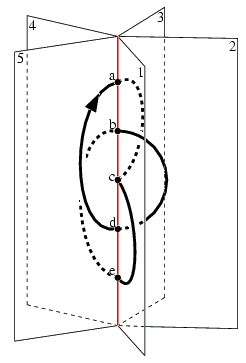
\includegraphics[width=0.2\linewidth]{MichaelImages/arc_index_fig1.png}
    \caption{Arc Presentation Trefoil}
    \label{fig:enter-label}
\end{figure}
\end{frame}

\begin{frame}{Arc Presentation and Arc Index}
\vspace{20px}
\begin{definition}
    The minimum number of pages required to represent a knot is called its arc index
\end{definition}

\begin{example}
    The arc index of a $(p,q)$ torus knot is $p+q$. This was shown using techniques from contact geometry.
\end{example}
\end{frame}

\begin{frame}[c]{Knot Game}
\begin{center}
    Before we start the proof we will play a quick game!
    The goal is to guess the correct knot inside the sponge.
\end{center}


\end{frame}

\begin{frame}[c]{Knots in The Menger Sponge}
We now give the proof that every knot can be found in a finite iteration of the merger sponge.
\begin{itemize}
    \item Given a knot $K$ we let $\{a_1, b_1\}, \dots, \{a_n, b_n\}$ be its arc presentation.
    \item Take an iteration of the Cantor set C, with at least $n$ endpoints and pick $n$ of these points $p_1, \dots p_k \in C$.
    \item We now re-write the arc presentation as $\{p_{a_1}, p_{b_1}\} \dots \{p_{a_n}, p_{b_n}\}$
    \item This does not change the knot!
\end{itemize}
\end{frame}

\begin{frame}[c]{Knots in The Menger Sponge}
\begin{itemize}
    \item We notice if $x_0 \in C$ then $(x_0, y,0)$ lies entirely on the front face of the sponge for $0 \leq y \leq 1$
    \item Similarly if $y_0 \in C$ $(x, y_0,0)$ lies entirely on the front face of the sponge for $0 \leq x \leq 1$
    \item We conclude the entire knot diagram induced by the given arc presentation lies on the front face of the sponge
\end{itemize}

\begin{figure}
    \centering
    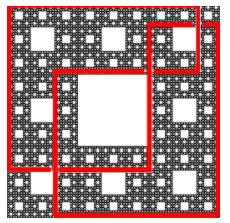
\includegraphics[width=0.2\linewidth]{KnotOnFace.png}
    \caption{\cite{broden2024knotsinsidefractals}}
    \label{fig:enter-label}
\end{figure}
\end{frame}

\begin{frame}[c]{Push Through the Sponge!}
The last big idea is to push the knot through the sponge
\begin{itemize}
    \item We draw the vertical lines on the front face and the horizontal lines on the back face.
    \item We connect them through the sponge.
    \item This is possible as the points $(x_0, y_0)$ were cantor dust points!
    \item The knot is our original knot as the projection onto the front face recovers our knot diagram.
\end{itemize}
\end{frame}

\section{Embedding into Sierpinski Tetrahedron}

\begin{frame}
	\frametitle{Difficulties}
	\begin{center}
	\begin{tabular}{|c|c|}
		\hline
		\textbf{Menger Sponge} & \textbf{Sierpinski Tetrahedron} \\
		\hline
		Easily understandable representation  & Difficulties caused by tetrahedrons \\
		\hline
		arc representation & ? \\
		\hline
	\end{tabular}
	\end{center}\\
	\\
	\onslide<2->
	Solution:
	\begin{itemize}
		\item Combinatorial representation of the Sierpinski Tetrahedron
		\item Pretzel knots
	\end{itemize}
	
\end{frame}

\begin{frame}
	\frametitle{Combinatorial representation of the Tetrahedron} % Changed from "Frame-titel"
	\begin{figure}[h]
		\centering
		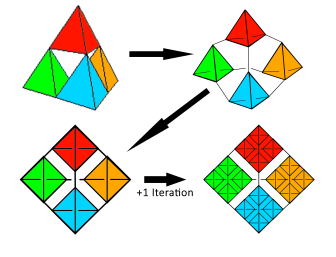
\includegraphics[width=0.5\linewidth]{images/CombRep1}
		\caption{Combinatorial representation of the Tetrahedron \cite{broden2024knotsinsidefractals}}
		\label{fig:enter-label}
	\end{figure}
\end{frame}

\begin{frame}
	\frametitle{Combinatorial representation of the Tetrahedron} % Changed from "Frame-titel"
	\begin{figure}[h]
		\centering
		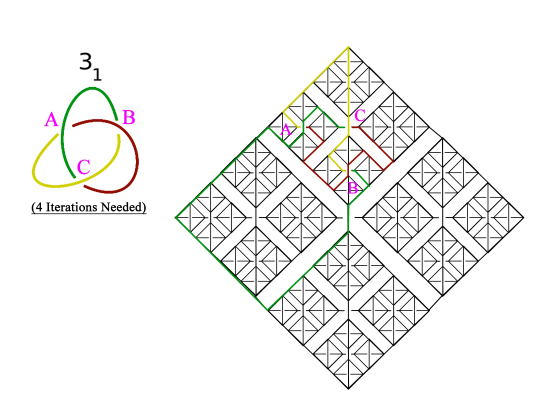
\includegraphics[width=0.5\linewidth]{images/CombRep2}
		\caption{Example $3^1$ knot \cite{broden2024knotsinsidefractals}}
		\label{fig:enter-label}
	\end{figure}
\end{frame}

\begin{frame}
	\frametitle{Combinatorial representation of the Tetrahedron} % Changed from "Frame-titel"
	\begin{figure}[h]
		\centering
		\includegraphics[width=0.5\linewidth]{images/CombRep3}
		\caption{Example $3^1$ knot \cite{broden2024knotsinsidefractals}}
		\label{fig:enter-label}
	\end{figure}
\end{frame}

\begin{frame}
	\frametitle{Sierpinski Tetrahedron} % Changed from "Frame-titel"
	\begin{theorem}
		All Pretzel Knots are inside a finite iteration of the Sierpinski Tetrahedron. \cite{broden2024knotsinsidefractals}
	\end{theorem}
	\onslide<2->
	\begin{proof}
		\begin{lemma}
			Every isolated helix can be put inside a finite iteration of the tetrahedron. \cite{broden2024knotsinsidefractals}
		\end{lemma}
		\onslide<3->
		To finish the proof they showed, that the helices can be connected as required.  
	\end{proof}
	\onslide<4->
	\begin{itemize}
		\item It is easy to follow that a certain Pretzel knot in which iteration can be embedded.
	\end{itemize}
\end{frame}

\begin{frame}
	\frametitle{Sierpinski Tetrahedron}
	\begin{figure}[h]
		\centering
		\includegraphics[width=1.0\linewidth]{images/Helix1}
		\caption{Helices in a certain iteration. \cite{broden2024knotsinsidefractals}}\label{Fig:Helix1}
	\end{figure}
\end{frame}

\begin{frame}
	\frametitle{Sierpinski Tetrahedron}
	\begin{figure}[!htb]
		\begin{minipage}{0.4\textwidth}
			\centering
			\includegraphics[width=1.0\linewidth]{images/SimplifiedPretzelKnot}
			\caption{Every Pretzel Knot can be simplified to the above form. \cite{broden2024knotsinsidefractals}}\label{Fig:SimplifiedPretzelKnot}
		\end{minipage}\hfill
		\begin{minipage}{0.6\textwidth}
			\centering
			\includegraphics[width=1.0\linewidth]{images/ConnectHelices}
			\caption{It is possible to connect the helices in the required order. \cite{broden2024knotsinsidefractals}}\label{Fig:ConnectHelices}
		\end{minipage}
	\end{figure}
\end{frame}

\begin{frame}
	\frametitle{Comparison between Fractals} % Changed from "Frame-titel"
	Denote with $M_n$ and $S_n$ the one-skeleton of the $n^{th}$ iteration of the Menger sponge and the Sierpinski Tetrahedron.\\
	Let $M(K)=\min{n}$, such that $K\subset M_n$. Similarly $S(K)=\min{n}, s.t. K\subset S_n$.\\
	\onslide<2->
	\begin{theorem}
		Let K be a not, then we have
		$$M(K)\leq S(K),$$
		whenever $S(K)$ is defined. \cite{broden2024knotsinsidefractals}
	\end{theorem}
	
	\onslide<3->
	\begin{proof}
		Shortly: The one-skeleton of the $i^{th}$ iteration of the Sierpinski Tetrahedron can be embedded into the one-skeleton of the $i^{th}$ iteration of the Menger Sponge. This embedding preserves the knot type.
	\end{proof}
\end{frame}

\begin{frame}
	\frametitle{Comparison between Fractals} % Changed from "Frame-titel"
	\begin{figure}[!htb]
		\begin{minipage}{0.48\textwidth}
			\centering
			\includegraphics[width=0.42\linewidth]{images/Comparison1}
			\caption{$S_0$ in $M_0$}\label{Fig:Data1}
		\end{minipage}\hfill
		\begin{minipage}{0.48\textwidth}
			\centering
			\includegraphics[width=0.42\linewidth]{images/Comparison2}
			\caption{$S_1$ in $M_1$}\label{Fig:Data2}
		\end{minipage}
	\end{figure}
	\onslide<2->
	What next?
	\onslide<3->
	\begin{itemize}
		\item To get $S_2$ in $M_2$: replace every $S_0$ in $S_1$ by $S_1.$
		\onslide<4->
		\item To get $S_{n+1}$ in $M_{n+1}$: replace every $S_0$ in $S_n$ by $S_1.$
		\onslide<5->
		\item Substitutions are in disjoint regions, so the embedding preserves the knot type.
	\end{itemize}
\end{frame}

\begin{frame}
	\frametitle{Open questions \cite{broden2024knotsinsidefractals}}
	\begin{itemize}
		\item Every knot can be embedded into the Sierpinski tetrahedron.
		\onslide<2->
		\begin{figure}[h]
			\centering
			\includegraphics[width=0.25\linewidth]{images/8_12}
			\caption{$8_{12}$ knot is not a Pretzel knot \cite{knotinfo}}\label{Fig:8_12}
		\end{figure}
		\onslide<3->
		\item Is there a fractal defined by iterative steps that doesn't admit all of the knots? If it is so, what does this tell us about the fractal?
	\end{itemize}
\end{frame}

\begin{frame}
\frametitle{Conclusion} % Changed from "Afsluitende frame"
\begin{itemize}
	\item Knot theory
	\item Fractals
	\item Intersection: Knots inside Fractals
	\item Open questions
\end{itemize}
\end{frame}


\begin{frame}[allowframebreaks]
    \frametitle{References}
%    \bibliography{ref}
    %\bibliographystyle{apalike}
     %adjust the fonts if there are too many references:
     %\tiny
     \printbibliography
\end{frame}

\begin{frame}
	\frametitle{Fantastic Knots and Where to Find Them}
	\begin{figure}[h]
		\centering
		\includegraphics[width=0.8\linewidth]{images/KnotTable}
		\caption{Knot table \cite{knotinfo}}
		\label{fig:enter-label}
	\end{figure}
\end{frame}



\end{document}